\section{Visualisierung}
\begin{figure}[ht]
\centering
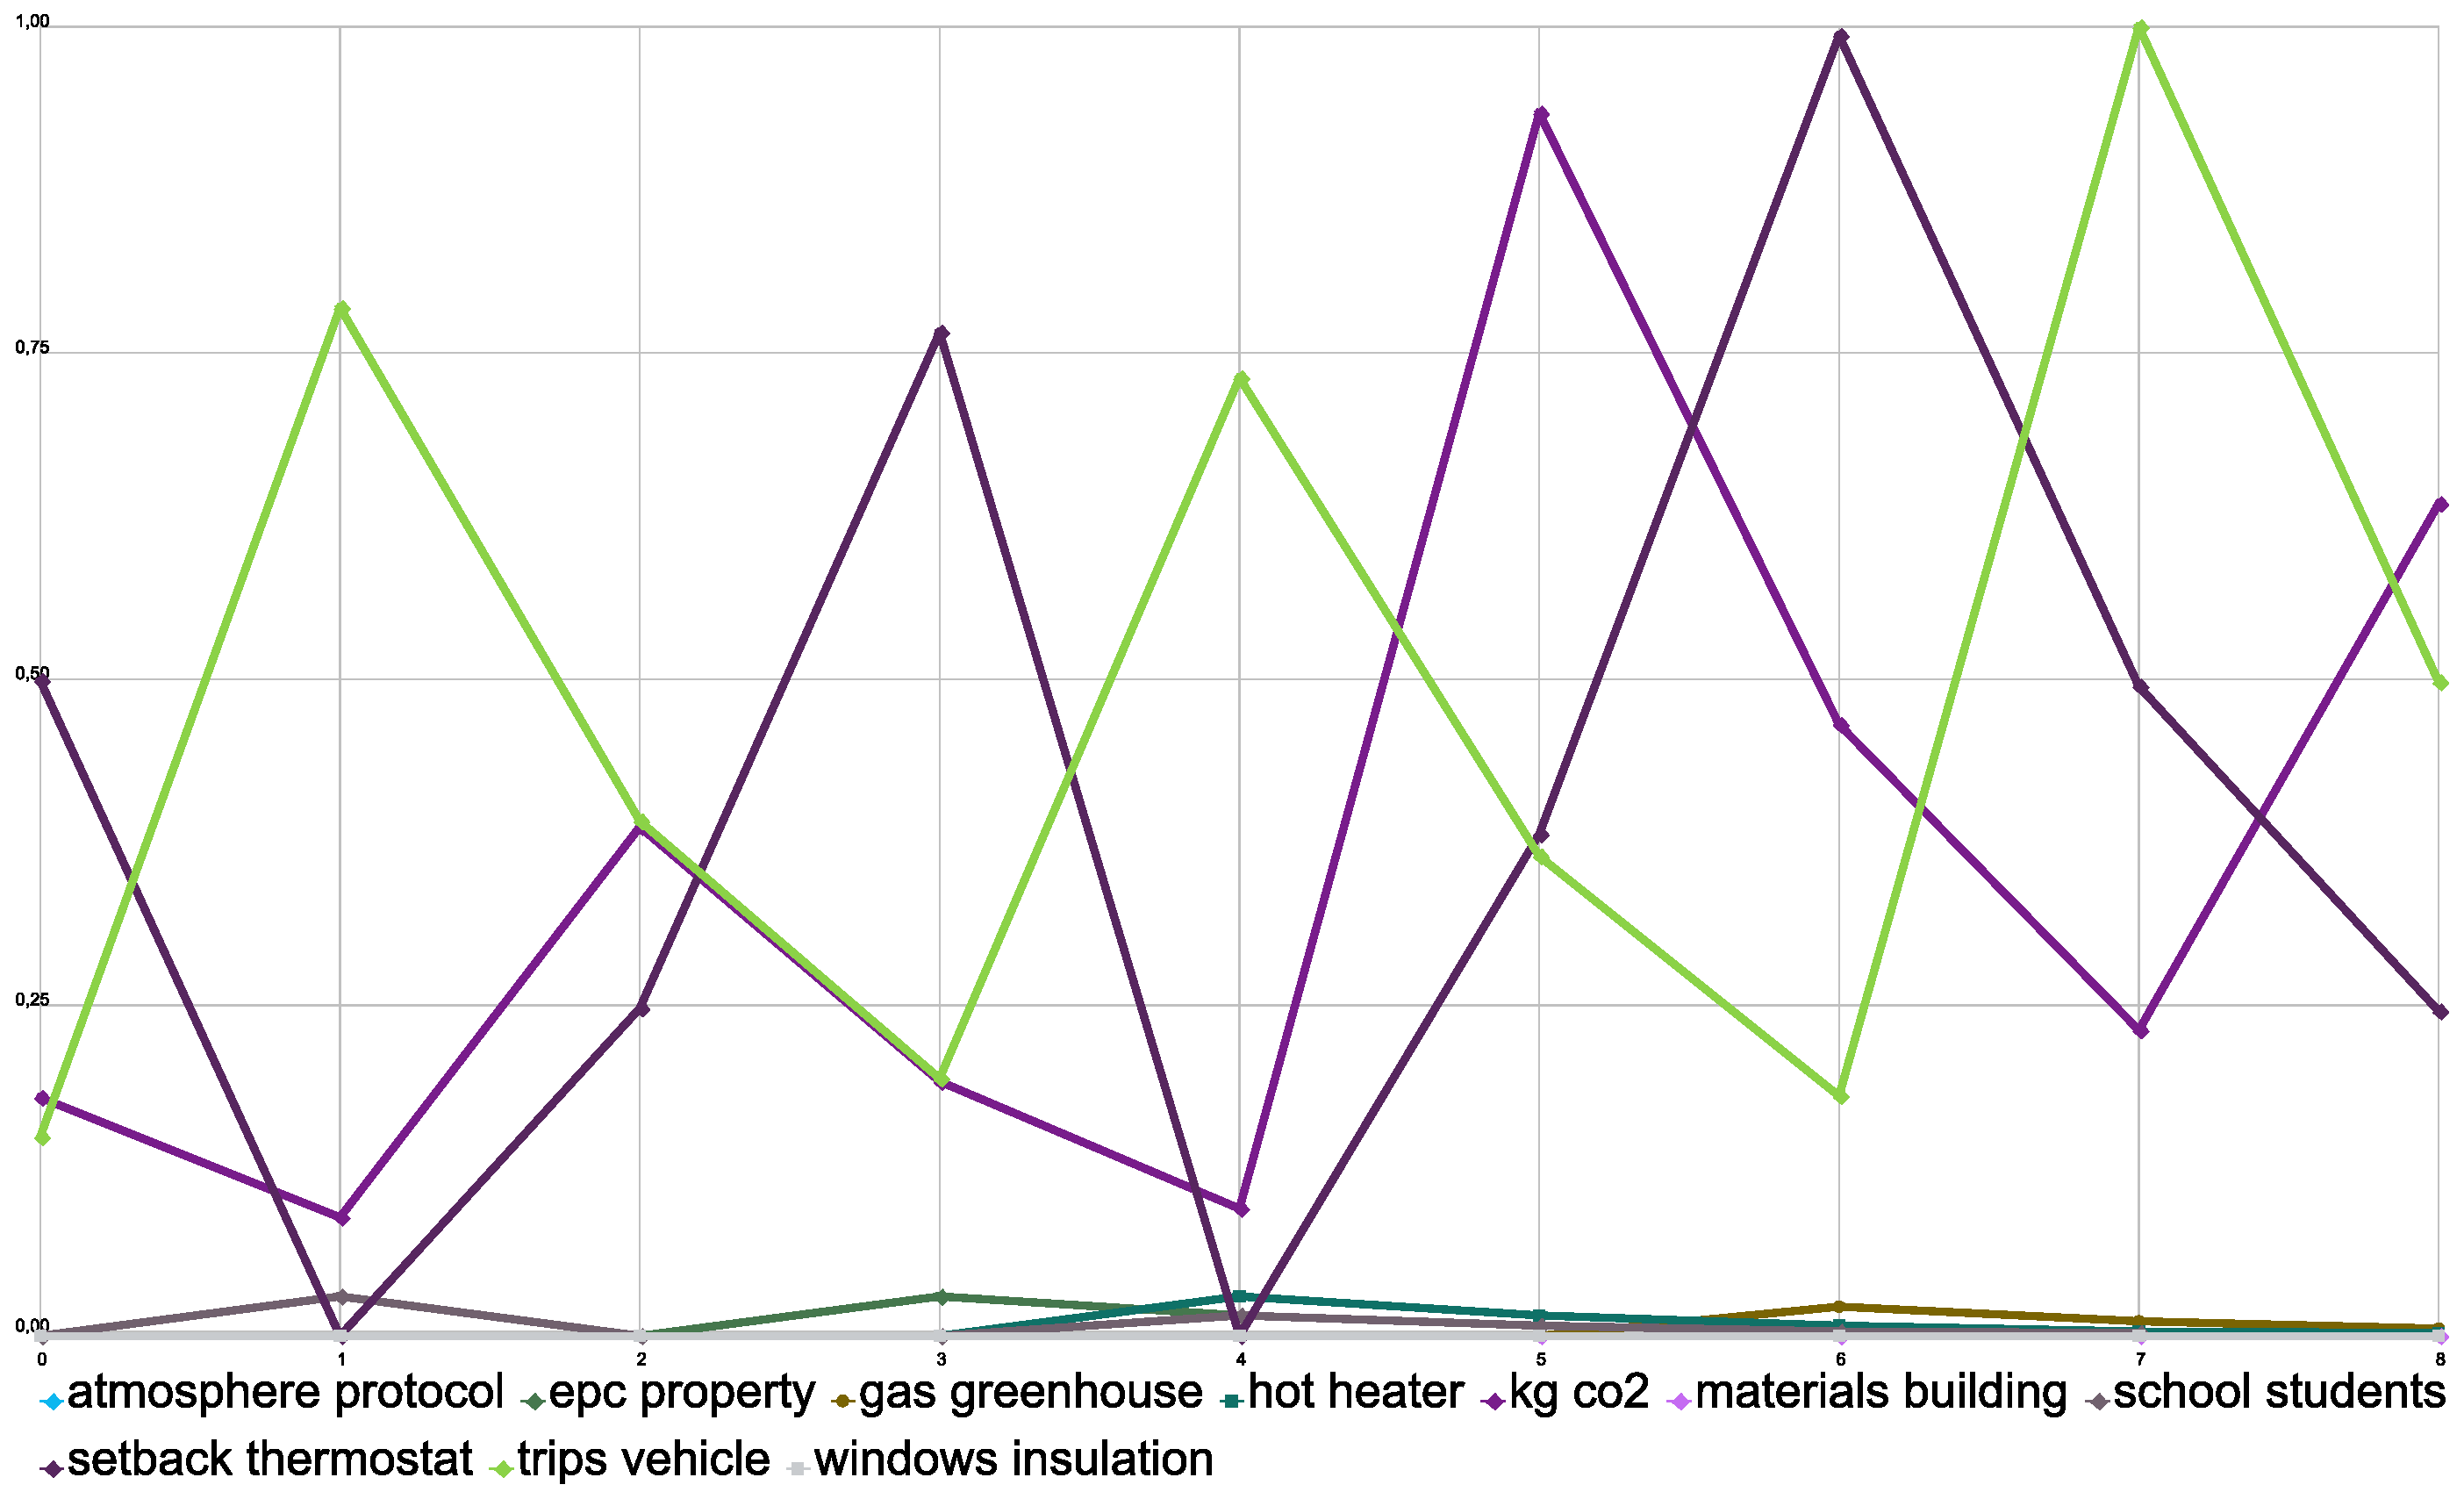
\includegraphics[width=\textwidth, height=0.5\textheight]{images/content/05_workflowTime/allInOne.eps} 
\caption{Alle Themenverläufe in einem Diagramm. Auf der X-Achse ist die Framezahl aufgetragen, auf der Y-Achse die normalisierte Zentralität}
\label{fig:allInOne}
\end{figure}

Für die Visualisierung der Themenverläufe wurde eine eigene Komponente entwickelt, die die Verläufe darstellt. Es wurden zwei Arten der Visualisierung implementiert. In der ersten Variante werden die Themenverläufe als Liniendiagramm in dasselbe Koordinatensystem eingezeichnet. Auf der X-Achse wird die laufende Framenummer abgetragen und auf der Y-Achse die normalisierte Zentralität. Jedes Thema wird durch eine eigene Linie repräsentiert. Welche Linie welches Thema repräsentiert wird als Beschriftung unterhalb des Diagramms eingeblendet (siehe Abbildung \ref{fig:allInOne}). 

\begin{figure}[ht]
\centering
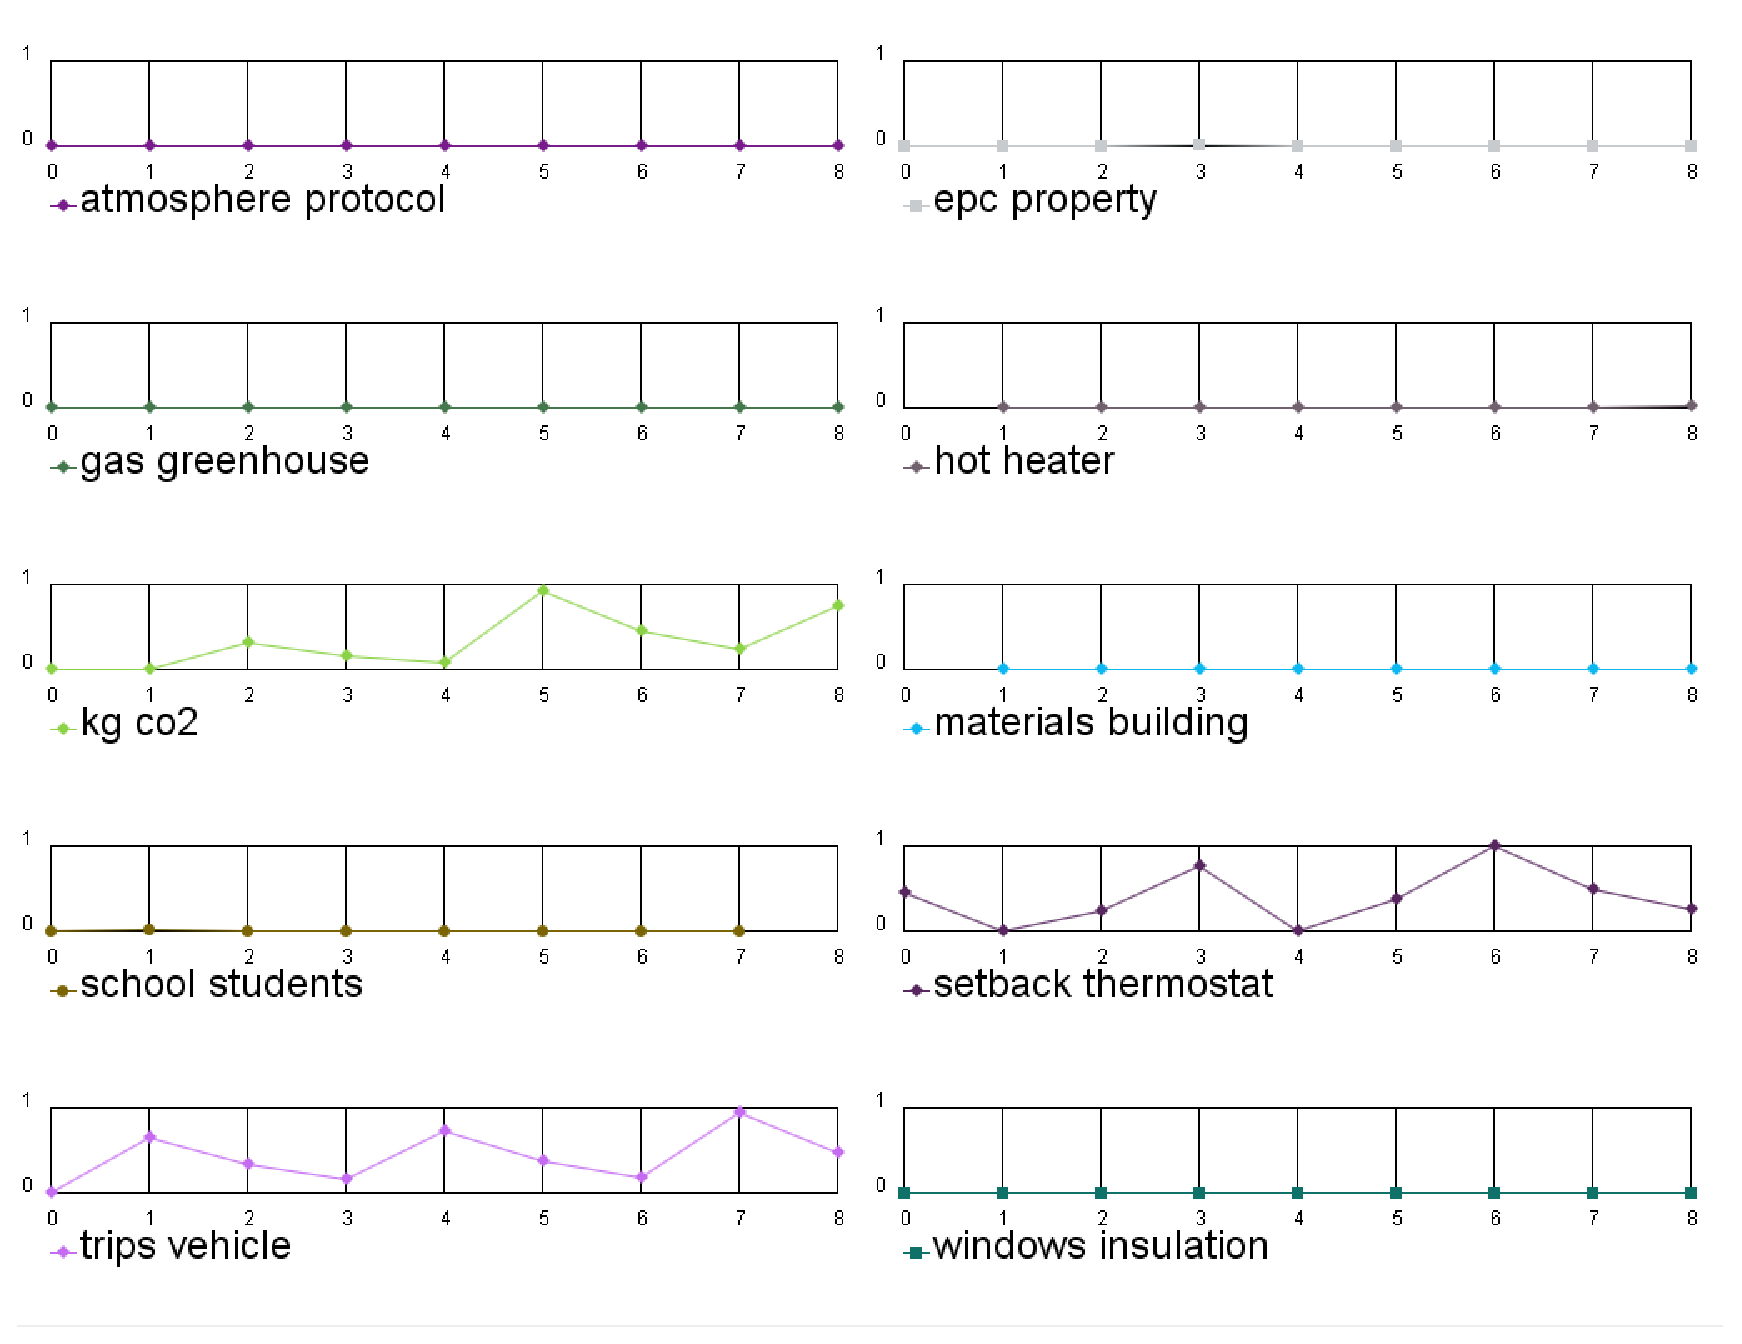
\includegraphics[width=\textwidth]{images/content/05_workflowTime/separatedViews.eps} 
\caption{Jeder Themenverlauf in einem eigenen Diagramm. Auf der X-Achse ist die Framezahl aufgetragen, auf der Y-Achse die normalisierte Zentralität}
\label{fig:separatedViews}
\end{figure}

Bei dieser Art der Visualisierung kann das Problem auftreten, dass die Prominenz der Themen nicht mehr differenziert werden kann, wenn viele Themen einen ähnlichen Verlauf haben, bzw. einen Verlauf auftritt, der viele andere Verläufe schneidet. Andererseits können bei Verläufen, in denen nicht viele Themen eine hohe Prominenz aufweisen, mit einem Blick die wichtigen Themen abgelesen werden und das Verhältnis zu den anderen Themen bestimmt werden.

In der zweiten Variante zeichnet man die Themenverläufe jeweils in ein eigenes Diagramm ein (siehe Abbildung \ref{fig:separatedViews}). Diese Diagramme werden dann in einer Matrix angeordnet. Diese Art der Visualisierung hat den Vorteil, dass man besser differenzieren kann, welche Themen wichtig sind. Jedoch ist die relative Zentralität eines Themas im Verhältnis zu anderen Themen schwieriger zu erkennen.
